\section{Overview}
\label{sec:Overview}
\thetool{} is designed to support the extraction of commits from different version control systems and various analyses of those extracted commits in any combination. For this purpose, it offers an open plug-in infrastructure implemented in Java. The core components of this infrastructure are the commit extractor, the internal data model, the commit analyzer, and the configuration file as illustrated in Figure~\ref{fig:Overview}. In this section, we will describe these components in detail.

\begin{figure}[h] % t für top, b = bottom, h = here
	\centering
		%trim={<left> <lower> <right> <upper>}
		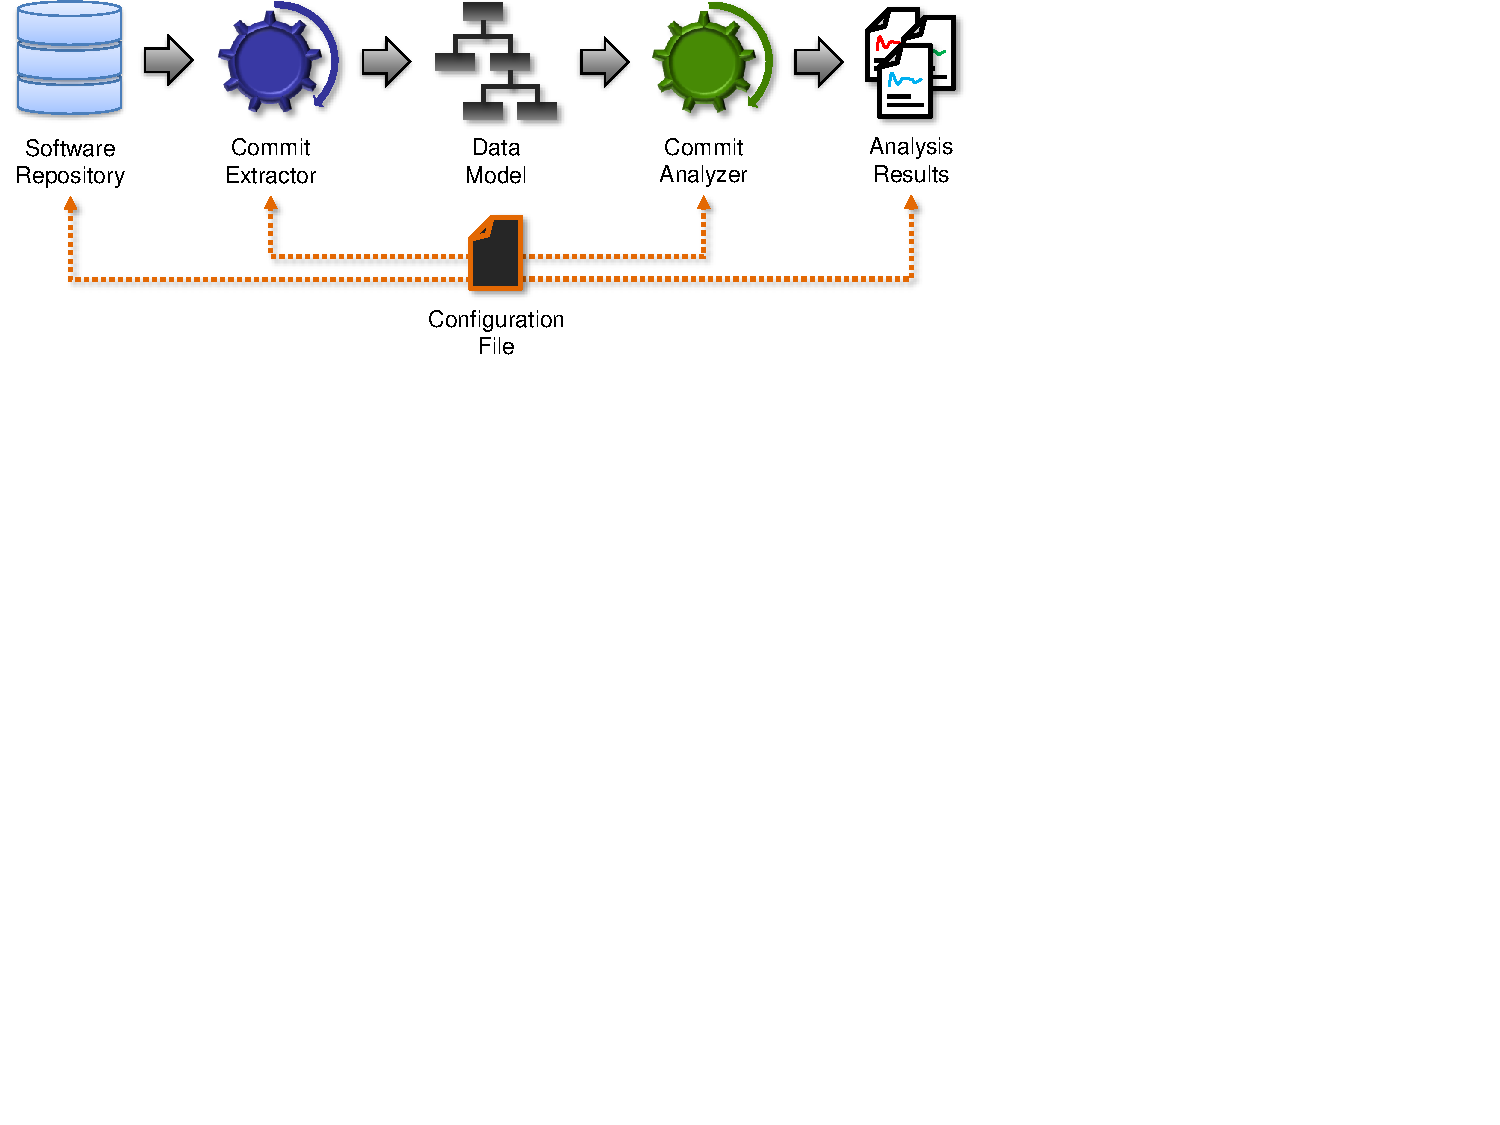
\includegraphics[width=\columnwidth,trim={0,2cm 13cm 9cm 0cm},clip]{inserts/comani_overview.pdf}
  \caption{\thetool{} overview}
	\label{fig:Overview}
\end{figure}

A \textbf{commit extractor} is a \thetool{} plug-in, which is responsible for the extraction of commits and their provision for the commit analysis as elements of the internal data. A commit extractor typically supports three extraction variants\footnote{While the respective methods need to be implemented by each commit extractor, developers are free to realize the required algorithms. Hence, we cannot guarantee that all extractors support all extraction variants. We recommend reading the description of the desired commit extractor for more information.} depending on the given sources from which the commits shall be extracted:

\begin{itemize}
\item \textit{Full repository extraction}: this variant forces the extraction of all commits of a software repository. This requires the definition of the location of the target repository as part of the configuration file.
\item \textit{Partial repository extraction}: instead of extracting all commits of a software repository, this variant allows the extraction of a predefined set of commits. Besides the location of the target repository, this requires the specification of an additional file, which contains a list of unique commit numbers (or hashes). Each line of this commit list file must contain exactly one commit number. Further, the author of the commit list file must ensure that the commit numbers specify commits of the target repository.
\item \textit{Single commit extraction}: the third variant offers an interactive mode, in which the content of a single commit can be passed on the command line as an input. It must be terminated by a last line only containing the string \texttt{!q!}. If this line is missing, the extraction will fail. Further, all lines after \texttt{!q!} will be ignored. However, the exact format of that string representing a single commit depends on the particular commit extractor. Please read the respective part of the documentation of the commit extractor in use for this information (typically defined in the \texttt{README.md} file). 
\end{itemize}

The available extractors are introduced in Section~\ref{sec:Installation}. Section~\ref{sec:Execution} describes their definition for a particular \thetool{} instance and the usage of the different extraction variants above. Further, Section~\ref{sec:CommitExtractorPlugins} explains the development of new extractor plug-ins for custom commit extraction capabilities.

The internal \textbf{data model} represents the conceptual interface between commit extractors and commit analyzers. It offers two main elements for representing commits: the \texttt{Commit} itself, which provides information, like its id (the commit number) or date, and the \texttt{ChangedArtifact} for storing the information about the artifacts changed by a specific commit. Hence, each commit typically contains a list of changed artifacts, which in turn contain information about their name and location as well as their content including the changed lines. A commit extractor creates instances of these elements based on the extracted commits from a target repository or the content of a commit passed as command line input. Section~\ref{sec:DataModel} provides further details about the internal data model and its elements.

The elements of the internal data model are input to a \textbf{commit analyzer}, which is a \thetool{} plug-in similar to a commit extractor. Depending on the core algorithm of the respective analysis, a commit analyzer may either wait until all commits are available or directly start processing at the time a commit is available. The infrastructure neither imposes any restriction on the way of processing nor on the analysis results. Hence, each commit analyzer has full control over its result creation. The only input it receives is an output directory in which the results can be stored. While the available analyzers are introduced in Section~\ref{sec:Installation}, their definition for and usage in a \thetool{} instance are described in Section~\ref{sec:Execution}. Section~\ref{sec:CommitAnalyzerPlugins} explains the development of this type of plug-ins in detail.

The \textbf{configuration file} in the lower part of Figure~\ref{fig:Overview} defines a particular setup of the commit extraction and analysis and, hence, a specific instance of \thetool{}. It consists of a set of configuration parameters for preparing the infrastructure (input and output locations, etc.) as well as defining the desired commit extractor and analyzer plug-ins. The infrastructure reads these parameters to configure \thetool{} prior to its actual execution. Section~\ref{sec:Execution} introduces the available configuration parameters and their definition for a particular \thetool{} instance.